\section{Описание модели АНПА} \label{sec:model_anpa}

Исследуемый объект контроля представляет собой АНПА, предназначенный для автономного поиска скоплений плонктона,
рыбных косяков или китов под водой путем испускания специализированной зондирующей посылки и ее анализа.
АНПА заключен в металлический корпус, внутри которого располагаются следующие составные части,
как показано на рисунке \ref{fig:model_anpa}.
\begin{center}
    \begin{figure}
        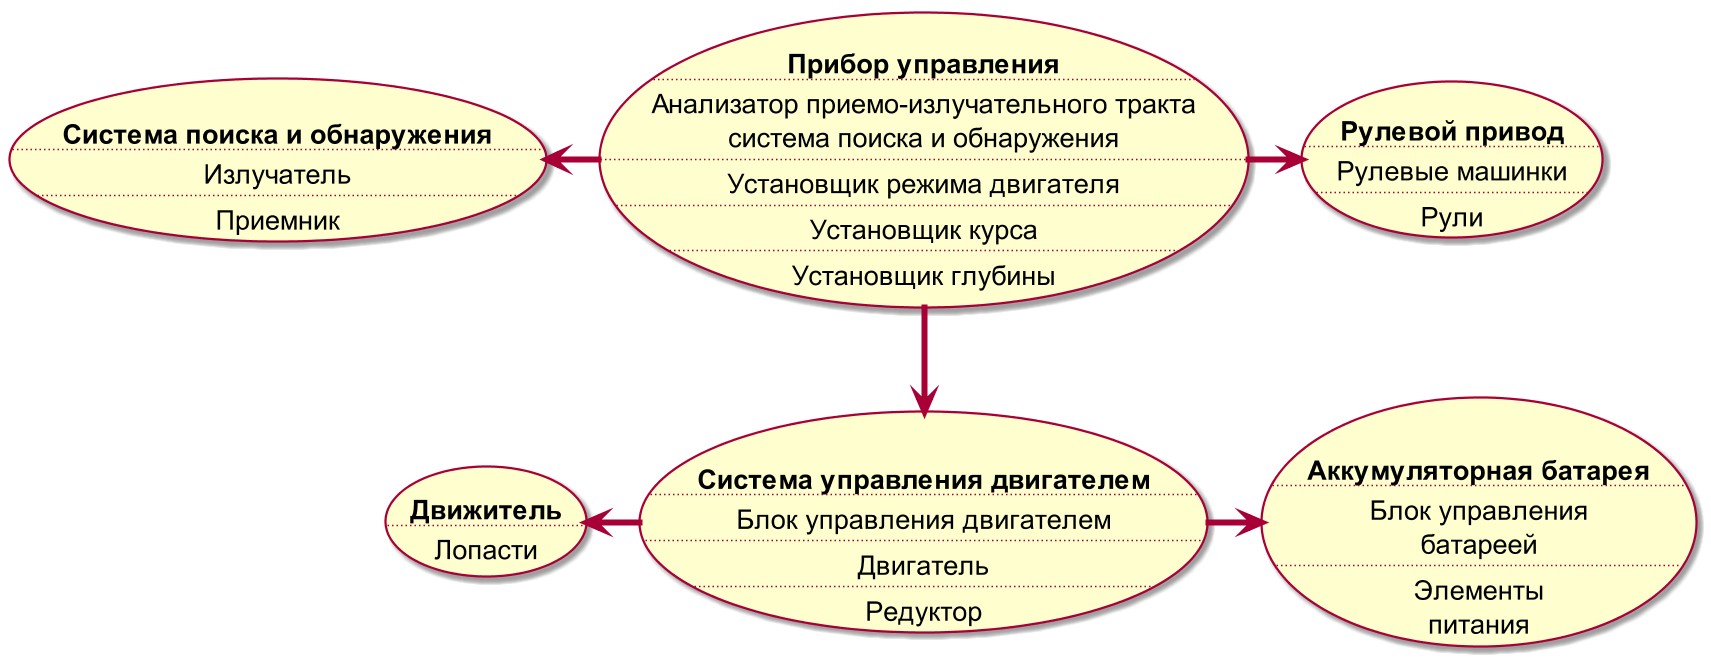
\includegraphics[width=.5\textwidth,keepaspectratio]{model_anpa}
        \caption{Декомпозиция материальной составляющей АНПА на составные части и взаимодействие между ними.}
            \label{fig:model_anpa}
    \end{figure}
\end{center}
В данной модели предполагается, что прибор управления является центральным управляющим узлом изделия,
на который возложены все функции принятия решений.

Связи \textbf{объект--функция--действие} АНПА показаны в таблице \ref{tbl:model_anpa} \cite{journal:vestnik_igeu:elizarova}.
%
\begin{landscape}
\begin{longtable}[c]{llm{.25\textwidth}||l|l|m{.25\textwidth}||llm{.25\textwidth}}
\caption{Декомпозиция организационной составляющей модели АНПА на \textbf{объекты}, \textbf{функции} и \textbf{действия}.}
\label{tbl:model_anpa_decompose}\\
\hline
\multicolumn{3}{|c||}{\textbf{Объекты}}                                                                                     & \multicolumn{3}{c||}{\textbf{Функции}}                                                                  & \multicolumn{3}{c|}{\textbf{Действия}}                                                                                                  \\ \hline
\endhead
%
\multicolumn{1}{|c|}{\textbf{1}}           & \multicolumn{1}{c|}{\textbf{2}} & \multicolumn{1}{c||}{\textbf{3}}            & \multicolumn{1}{c|}{\textbf{1}}   & \multicolumn{1}{c|}{\textbf{2}} & \multicolumn{1}{c||}{\textbf{3}} & \multicolumn{1}{c|}{\textbf{1}}           & \multicolumn{1}{c|}{\textbf{2}} & \multicolumn{1}{c|}{\textbf{3}}                           \\ \hline
\multicolumn{1}{|l|}{\multirow{2}{*}{СПО}} & \multicolumn{1}{l|}{1}          & Излучатель                                  & \multirow{5}{*}{Движение}         & 1                               & Вперед                           & \multicolumn{1}{l|}{\multirow{3}{*}{ПУ}}  & \multicolumn{1}{l|}{1}          & \multicolumn{1}{l|}{Пеленгация целей}                     \\ \cline{2-3} \cline{5-6} \cline{8-9} 
\multicolumn{1}{|l|}{}                     & \multicolumn{1}{l|}{2}          & Приемник                                    &                                   & 2                               & Вправо                           & \multicolumn{1}{l|}{}                     & \multicolumn{1}{l|}{2}          & \multicolumn{1}{l|}{Коррекция курса}                      \\ \cline{1-3} \cline{5-6} \cline{8-9} 
\multicolumn{1}{|l|}{\multirow{4}{*}{ПУ}}  & \multicolumn{1}{l|}{3}          & Анализатор приемо-излучательного тракта СПО &                                   & 3                               & Влево                            & \multicolumn{1}{l|}{}                     & \multicolumn{1}{l|}{3}          & \multicolumn{1}{l|}{Коррекция глубины}                    \\ \cline{2-3} \cline{5-9} 
\multicolumn{1}{|l|}{}                     & \multicolumn{1}{l|}{4}          & Установщик режима двигателя                 &                                   & 4                               & Вверх                            & \multicolumn{1}{l|}{\multirow{2}{*}{АКБ}} & \multicolumn{1}{l|}{4}          & \multicolumn{1}{l|}{Хранение электроэнергии}              \\ \cline{2-3} \cline{5-6} \cline{8-9} 
\multicolumn{1}{|l|}{}                     & \multicolumn{1}{l|}{5}          & Установщик курса                            &                                   & 5                               & Вниз                             & \multicolumn{1}{l|}{}                     & \multicolumn{1}{l|}{5}          & \multicolumn{1}{p{.25\textwidth}|}{Доставка электроэнергии потребителям} \\ \cline{2-9} 
\multicolumn{1}{|l|}{}                     & \multicolumn{1}{l|}{6}          & Установщик глубины                          & \multirow{5}{*}{Питание}          & 6                               & СПО                              & \multicolumn{1}{l|}{Д}                    & \multicolumn{1}{l|}{6}          & \multicolumn{1}{l|}{Толкает водную среду}                 \\ \cline{1-3} \cline{5-9} 
\multicolumn{1}{|l|}{\multirow{3}{*}{СУД}} & \multicolumn{1}{l|}{7}          & БУД                                         &                                   & 7                               & ПУ                               &                                           &                                 &                                                           \\ \cline{2-3} \cline{5-6}
\multicolumn{1}{|l|}{}                     & \multicolumn{1}{l|}{8}          & Двигатель                                   &                                   & 8                               & СУД                              &                                           &                                 &                                                           \\ \cline{2-3} \cline{5-6}
\multicolumn{1}{|l|}{}                     & \multicolumn{1}{l|}{9}          & Редуктор                                    &                                   & 9                               & РП                               &                                           &                                 &                                                           \\ \cline{1-3} \cline{5-6}
\multicolumn{1}{|l|}{\multirow{2}{*}{РП}}  & \multicolumn{1}{l|}{10}         & РМ                                          &                                   & 10                              & Д                                &                                           &                                 &                                                           \\ \cline{2-6}
\multicolumn{1}{|l|}{}                     & \multicolumn{1}{l|}{11}         & Рули                                        & \multirow{2}{*}{Обнаружение}      & 11                              & Излучение зондирующей посылки    &                                           &                                 &                                                           \\ \cline{1-3} \cline{5-6}
\multicolumn{1}{|l|}{Д}                    & \multicolumn{1}{l|}{12}         & Лопасти                                     &                                   & 12                              & Прием отраженого сигнала         &                                           &                                 &                                                           \\ \cline{1-6}
\multicolumn{1}{|l|}{\multirow{2}{*}{АКБ}} & \multicolumn{1}{l|}{13}         & БУБ                                         & \multirow{4}{*}{Принятие решений} & 13                              & Изменить скорость движения       &                                           &                                 &                                                           \\ \cline{2-3} \cline{5-6}
\multicolumn{1}{|l|}{}                     & \multicolumn{1}{l|}{14}         & Модули питания                              &                                   & 14                              & Изменить курс                    &                                           &                                 &                                                           \\ \cline{1-3} \cline{5-6}
                                           &                                 &                                             &                                   & 15                              & Изменить глубину хода            &                                           &                                 &                                                           \\ \cline{5-6}
                                           &                                 &                                             &                                   & 16                              & Изменить тип зондирующей посылки &                                           &                                 &                                                           \\ \cline{4-6}
\end{longtable}
\end{landscape}
%
Исходя из данных, представленных в таблице \ref{tbl:model_anpa},
строятся матрицы $A, B$:
%
\begin{equation}
    A = \begin{pmatrix}
    0 &   0 &   0 &   0 &   0 &   1 &   0 &   0 &   0 &   0 &   1 &   0 &   0 &   0 &   0 &   0 \\
    0 &   0 &   0 &   0 &   0 &   1 &   0 &   0 &   0 &   0 &   0 &   1 &   0 &   0 &   0 &   0 \\
    0 &   0 &   0 &   0 &   0 &   1 &   1 &   0 &   0 &   0 &   0 &   1 &   0 &   0 &   0 &   1 \\
    0 &   0 &   0 &   0 &   0 &   0 &   0 &   1 &   0 &   1 &   0 &   0 &   0 &   0 &   0 &   0 \\
    0 &   1 &   1 &   0 &   0 &   0 &   0 &   0 &   0 &   0 &   1 &   0 &   0 &   1 &   0 &   1 \\
    0 &   0 &   0 &   1 &   1 &   0 &   0 &   0 &   0 &   0 &   0 &   0 &   0 &   0 &   1 &   0 \\
    0 &   0 &   0 &   0 &   0 &   1 &   0 &   0 &   0 &   0 &   0 &   0 &   1 &   0 &   0 &   0 \\
    0 &   0 &   0 &   0 &   0 &   1 &   0 &   0 &   0 &   0 &   0 &   0 &   1 &   0 &   0 &   0 \\
    0 &   0 &   0 &   0 &   0 &   0 &   0 &   0 &   0 &   1 &   0 &   0 &   0 &   0 &   0 &   0 \\
    1 &   1 &   1 &   1 &   1 &   0 &   0 &   0 &   0 &   0 &   0 &   0 &   0 &   1 &   1 &   0 \\
    1 &   1 &   1 &   1 &   1 &   0 &   0 &   0 &   0 &   0 &   0 &   0 &   0 &   1 &   1 &   0 \\
    0 &   0 &   0 &   0 &   0 &   0 &   0 &   0 &   0 &   0 &   0 &   0 &   0 &   1 &   1 &   0 \\
    0 &   0 &   0 &   0 &   0 &   1 &   1 &   1 &   1 &   1 &   1 &   0 &   0 &   0 &   0 &   0 \\
    0 &   0 &   0 &   0 &   0 &   0 &   0 &   0 &   0 &   0 &   1 &   1 &   0 &   0 &   0 &   0 \\
    \end{pmatrix}\,,
    
    B = \begin{pmatrix}
        0 & 0 & 0 & 0 & 0 & 1 \\
        0 & 1 & 0 & 0 & 0 & 0 \\
        0 & 1 & 0 & 0 & 0 & 0 \\
        0 & 0 & 1 & 0 & 0 & 0 \\
        0 & 0 & 1 & 0 & 0 & 0 \\
        0 & 0 & 0 & 1 & 1 & 0 \\
        0 & 0 & 0 & 1 & 1 & 0 \\
        0 & 0 & 0 & 1 & 1 & 0 \\
        0 & 0 & 0 & 1 & 1 & 0 \\
        0 & 0 & 0 & 1 & 1 & 0 \\
        1 & 0 & 0 & 0 & 1 & 0 \\
        1 & 1 & 0 & 0 & 0 & 0 \\
        0 & 1 & 1 & 0 & 0 & 1 \\
        0 & 1 & 0 & 0 & 0 & 1 \\
        0 & 0 & 1 & 0 & 0 & 1 \\
        1 & 0 & 0 & 0 & 1 & 0 \\
    \end{pmatrix}\,.
\end{equation}

В результате умножения матриц $A$ и $B$ получаем матрицу $C_1$ размера $(6\times14)$,
которая определяет использование сущностей материальной составляющей предметной области действий, найденных через функции:

\begin{equation}
    C_1 = A \times B = \begin{pmatrix}
        1 & 0 & 0 & 1 & 2 & 0 \\
        1 & 1 & 0 & 1 & 1 & 0 \\
        2 & 1 & 0 & 2 & 3 & 0 \\
        0 & 0 & 0 & 2 & 2 & 0 \\
        2 & 3 & 0 & 0 & 2 & 1 \\
        0 & 0 & 3 & 0 & 0 & 1 \\
        0 & 1 & 1 & 1 & 1 & 1 \\
        0 & 1 & 1 & 1 & 1 & 1 \\
        0 & 0 & 0 & 1 & 1 & 0 \\
        0 & 3 & 3 & 0 & 0 & 3 \\
        0 & 3 & 3 & 0 & 0 & 3 \\
        0 & 1 & 1 & 0 & 0 & 2 \\
        1 & 0 & 0 & 5 & 6 & 0 \\
        2 & 1 & 0 & 0 & 1 & 0 \\
    \end{pmatrix}\,.
\end{equation}

Если $c_{1ik} = 0$, то сущность с номером $i$ не используется в функции с номером $k$ данной функции,
а если $c_{1ik} \ne 0$, то используется.

Построчное суммирование элементов матрицы $C_1$ получаем матрицу $C_2$, показывающую количественные характеристики
использования сущностей материальной составляющей предметной области в функциях:

\begin{equation*}
    C_2 = \begin{pmatrix}
        c_{21} = \sum_{j=1}^l c_{11j} \\
        \ldots \\
        c_{2m} = \sum_{j=1}^l c_{1mj} \\
    \end{pmatrix} 
    =
    \begin{pmatrix}
        4 \\
        4 \\
        8 \\
        4 \\
        8 \\
        4 \\
        5 \\
        5 \\
        2 \\
        9 \\
        9 \\
        4 \\
        12 \\
        4 \\
    \end{pmatrix}
\end{equation*}
где $c_{2i}$ количество функций, в которых используется данная сущность.

Делением матрицы $C_2$ на число $l = 6$, равное количеству действий в функциональной модели, получаем матрицу $C_3$,
содержащую относительные коэффициенты использования сущностей в действиях:
\begin{equation}
    C_3 = C_2 / l = \begin{pmatrix}
        0,67 \\
        0,67 \\
        1,33 \\
        0,67 \\
        1,33 \\
        0,67 \\
        0,83 \\
        0,83 \\
        0,33 \\
        \textbf{1,50} \\
        \textbf{1,50} \\
        0,67 \\
        \textbf{2,00} \\
        0,67 \\
    \end{pmatrix}\,.
\end{equation}
Установив пороговое значение $K_{min} = 1.5$ получаем, что общесистемными являются
\textit{рулевые машинки (1.5), рулевой привод (1.5) и блок управления батареей (2.0)}.
